\chapter[Analiza tematu: podstawy i specyfika transkrypcji gitarowej]{Analiza tematu: teoretyczne podstawy transkrypcji muzycznej i specyfika transkrypcji gitarowej}
\label{chap:analiza_tematu}

Rozdział pierwszy wprowadził w~ogólną problematykę automatycznej transkrypcji muzycznej (ATM) oraz zarysował specyficzne wyzwania związane z~muzyką gitarową. Niniejszy rozdział stanowi rozwinięcie podstaw teoretycznych, które są niezbędne do pełnego zrozumienia podejmowanego problemu oraz zaprojektowanego rozwiązania. Skupia się on na szczegółowej analizie dźwięku muzycznego, jego cyfrowej reprezentacji oraz metodach stosowanych w~ATM, kładąc fundament pod dalsze, bardziej techniczne części pracy.

\section{Sprecyzowanie problemu badawczego}
\label{sec:definicja_problemu_atm}

Jak wskazano we wstępie, proces ATM polega na przekształceniu sygnału audio na jego symboliczną reprezentację, taką jak format piano-roll czy standardowy zapis nutowy~\autocite{KlapuriDavy2006SignalProcessing,Benetos2019AutomaticMusicTranscription}. W~kontekście niniejszej pracy, problem ten zostaje sprecyzowany jako \textbf{automatyczna transkrypcja gitarowa na zapis tabulaturowy (GTT)} (ang. \textit{Guitar Tablature Transcription}). Zadanie GTT wykracza poza prostą identyfikację wysokości i~czasu trwania dźwięków, ponieważ obejmuje również ich precyzyjne przypisanie do konkretnych strun i~progów na gryfie gitary~\autocite{Wiggins2019TabCNN}. Ponadto, pełna transkrypcja tabulaturowa dąży do rozpoznania technik artykulacyjnych charakterystycznych dla gitary, takich jak podciągnięcia strun (ang. \textit{bends}), młoteczkowanie (ang. \textit{hammer-on}), odrywanie (ang. \textit{pull-off}) czy wibrato (ang. \textit{vibrato})~\autocite{Reboursiere2011GuitarController}, które są kluczowe dla wiernego odtworzenia utworu.

Mimo znaczącego potencjału aplikacyjnego, należy zauważyć, że obecne systemy ATM mogą nie zawsze oferować przewagę w~każdym scenariuszu, np. w~kontekstach etnomuzykologicznych, gdzie dla doświadczonych transkrybentów krytyczna jest precyzja notacji rytmicznej~\autocite{Holzapfel2019Ethnomusicology}.
\section{Podstawy teoretyczne: dźwięk muzyczny i jego cyfrowa reprezentacja}
\label{sec:podstawy_teoretyczne_dzwiek}

Zrozumienie procesów leżących u~podstaw automatycznej transkrypcji muzycznej wymaga uprzedniego zapoznania się z~właściwościami dźwięku muzycznego oraz sposobami jego cyfrowej reprezentacji i~analizy. Niniejsza sekcja przybliża te kluczowe koncepcje.

\subsection{Percepcyjne i fizyczne atrybuty dźwięku muzycznego}
\label{ssec:atrybuty_dzwieku}

Dźwięk muzyczny, z~perspektywy percepcji, charakteryzowany jest przez cztery podstawowe atrybuty: wysokość, głośność, barwę i~czas trwania~\autocite{KlapuriDavy2006SignalProcessing}. Wysokość jest bezpośrednio związana z~częstotliwością podstawową ($F_0$) drgań źródła dźwięku. Głośność to subiektywna ocena natężenia dźwięku. Barwa pozwala odróżnić dźwięki o~tej samej wysokości i~głośności, lecz pochodzące z~różnych instrumentów lub generowane różnymi technikami; jest ona ściśle powiązana ze spektrum harmonicznym dźwięku (rozkładem i~względnymi amplitudami składowych harmonicznych) oraz jego obwiednią czasową. Czas trwania definiuje, jak długo dźwięk jest postrzegany. Obwiednia amplitudy dźwięku, często modelowana jako ADSR (ang. \textit{Attack, Decay, Sustain, Release}; atak, zanikanie, podtrzymanie, wybrzmiewanie), odgrywa kluczową rolę w~kształtowaniu charakteru brzmieniowego, zwłaszcza dla instrumentów szarpanych, takich jak gitara~\autocite{KlapuriDavy2006SignalProcessing}. Jej schematyczną wizualizację przedstawia rysunek~\ref{fig:adsr}. Fazy ataku (narastania), początkowego zaniku, podtrzymania i~końcowego wybrzmiewania definiują dynamiczny profil dźwięku, przy czym dla gitary fazy zaniku i~wybrzmiewania są szczególnie złożone i~zależne od instrumentu oraz techniki gry.

\begin{figure}[H]
    \centering
    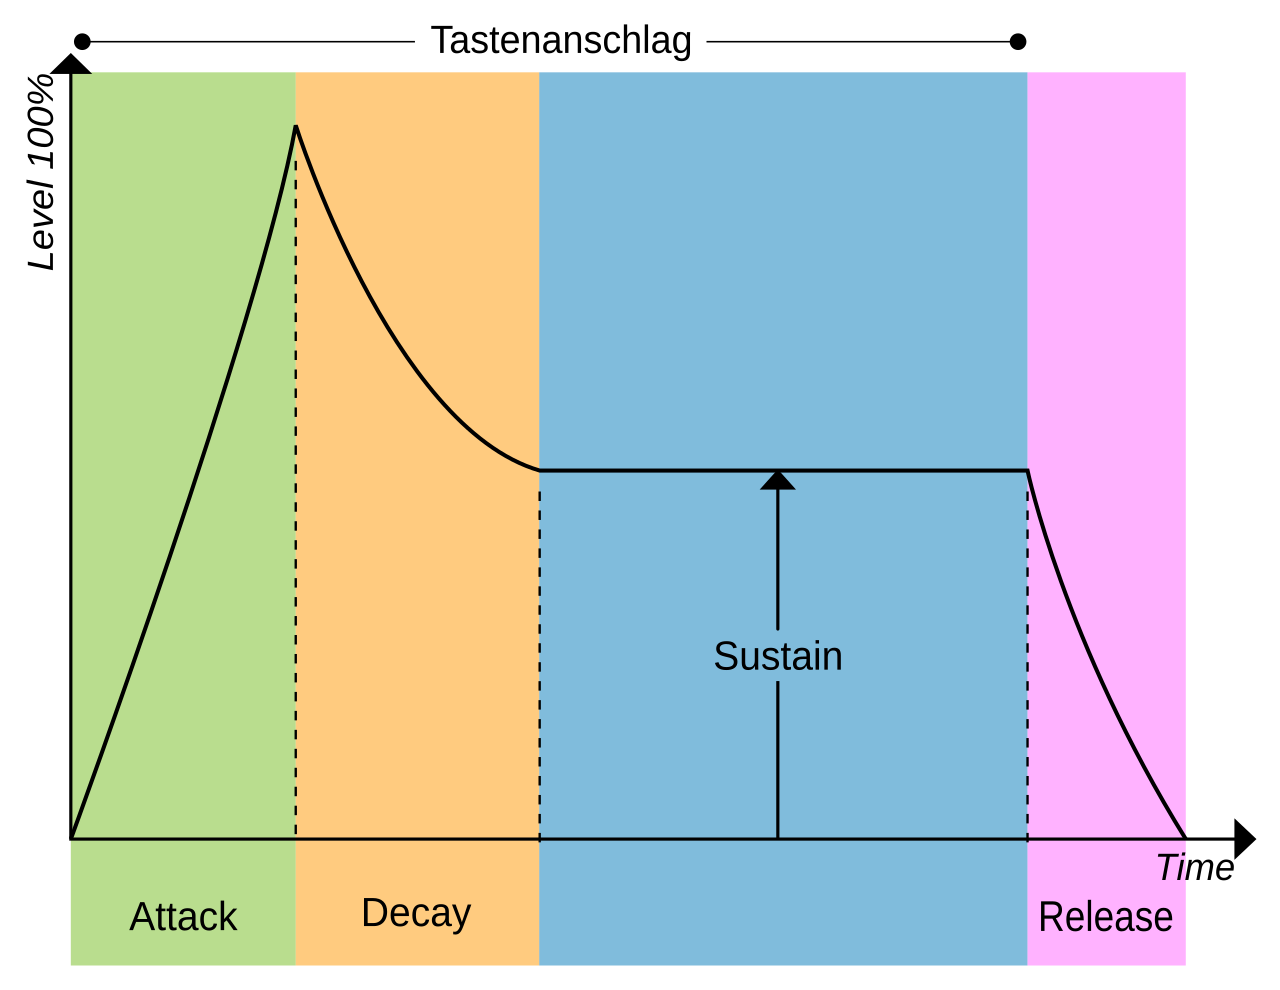
\includegraphics[width=0.8\textwidth]{fig/fig_2_5.png}
    \caption{Schematyczna wizualizacja obwiedni dźwięku ADSR (oś pionowa: amplituda, oś pozioma: czas)~\autocite{wiki:adsr}.}
    \label{fig:adsr}
\end{figure}

\subsection{Reprezentacja sygnału audio w dziedzinie czasu i częstotliwości}
\label{ssec:reprezentacja_czas_czestotliwosc}

Cyfrowy sygnał audio jest sekwencją próbek reprezentujących amplitudę fali akustycznej w~kolejnych, dyskretnych punktach czasu~\autocite{KlapuriDavy2006SignalProcessing}. Analiza wyłącznie w~dziedzinie czasu nie ujawnia jednak w~pełni struktury muzycznej sygnału. Kluczowa jest analiza częstotliwościowa, pozwalająca zidentyfikować składowe częstotliwościowe. Przejście z~dziedziny czasu do dziedziny częstotliwości realizowane jest za pomocą transformaty Fouriera, która dekomponuje sygnał na sumę składowych sinusoidalnych o~różnych częstotliwościach i~amplitudach, tworząc jego widmo częstotliwościowe~\autocite{KlapuriDavy2006SignalProcessing}. Dyskretna transformata Fouriera (DFT) jest podstawowym narzędziem tej analizy. Dla skończonego ciągu próbek sygnału~$x_n$ o~długości~N, jej k-ty współczynnik~$X_k$ jest zdefiniowany wzorem~(\ref{eq:dft}):
\begin{equation}
    X_k = \sum_{n=0}^{N-1} x_n \cdot e^{-i\frac{2\pi}{N}kn}
    \label{eq:dft}
\end{equation}
gdzie $n$ jest indeksem próbki w~dziedzinie czasu, $k$ jest indeksem częstotliwości, a~$i$ jest jednostką urojoną. Działanie transformaty ilustruje rysunek~\ref{fig:fig_2_1}.

\begin{figure}[!htbp]
    \centering
    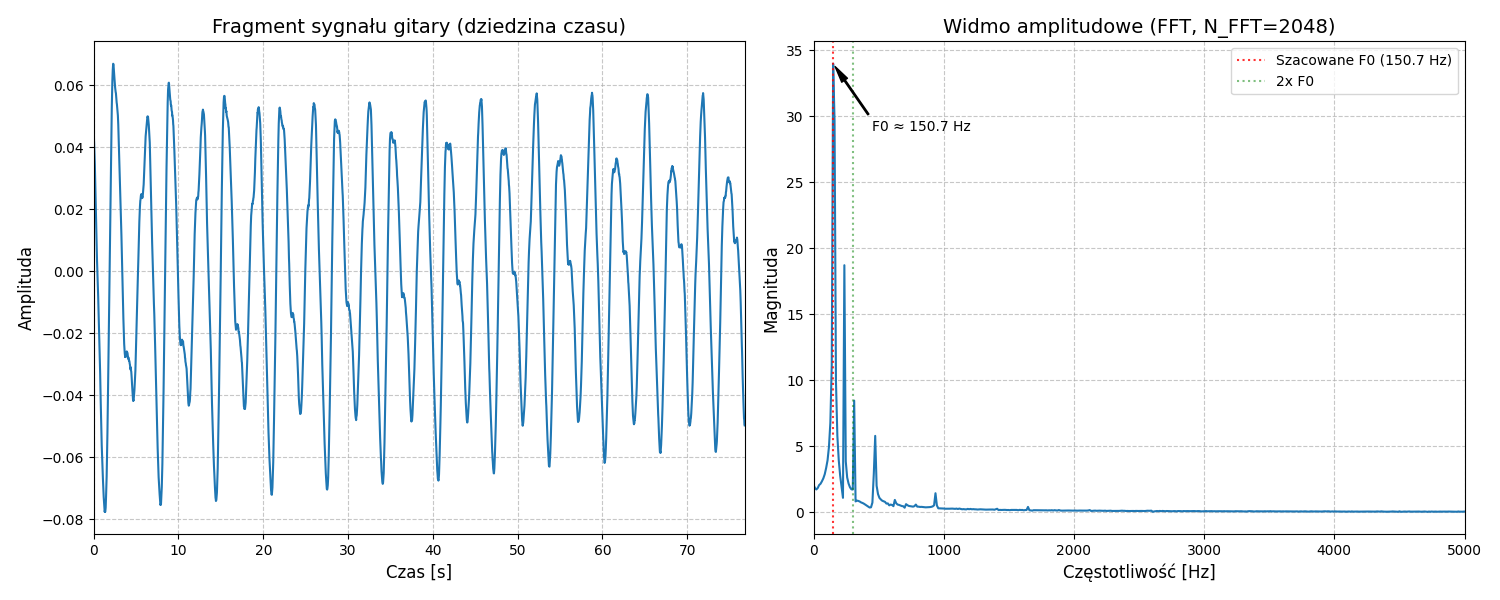
\includegraphics[width=\textwidth]{fig/fig_2_1.png}
    \caption{Po lewej: fragment sygnału audio pojedynczego dźwięku gitary w~dziedzinie czasu (oś pionowa: amplituda (wartość znormalizowana), oś pozioma: czas w~próbkach). Po prawej: odpowiadające mu widmo amplitudowe (oś pionowa: magnituda (jednostki względne), oś pozioma: częstotliwość w~Hz), ukazujące częstotliwość podstawową ($F_0$) oraz jej kolejne alikwoty (składowe harmoniczne).}
    \label{fig:fig_2_1}
\end{figure}

\subsection{Analiza czasowo-częstotliwościowa i jej znaczenie dla ATM}
\label{ssec:analiza_czas_czestotliwosc}

Charakterystyki częstotliwościowe muzyki zmieniają się w~czasie, dlatego w~zastosowaniach ATM niezbędne są metody analizy czasowo-częstotliwościowej. Podstawową techniką jest krótkoczasowa transformata Fouriera (ang. \textit{Short-Time Fourier Transform}, STFT), która polega na sekwencyjnej analizie Fouriera krótkich, najczęściej nakładających się na siebie segmentów sygnału~\autocite{KlapuriDavy2006SignalProcessing,BurletHindle2017IsolatedGuitarTranscription}. Wynikiem STFT jest spektrogram – dwuwymiarowa reprezentacja energii sygnału w~funkcji czasu i~częstotliwości, która stanowi podstawę dla wielu systemów ATM. Należy pamiętać o~nieodłącznym kompromisie STFT między rozdzielczością czasową a~częstotliwościową, wynikającym z~zasady nieoznaczoności. Kluczowym ograniczeniem tej metody w~kontekście muzycznym jest jej stała rozdzielczość częstotliwościowa, co oznacza, że pasma częstotliwości mają identyczną szerokość (np. w~hercach) na całej skali. Nie odpowiada to logarytmicznej naturze ludzkiej percepcji wysokości dźwięku.

\begingroup
\sloppy
W odpowiedzi na to ograniczenie opracowano alternatywne reprezentacje, lepiej dostosowane do specyfiki sygnału muzycznego. Jedną z~nich jest transformata Constant-Q (ang. \textit{Constant-Q Transform}, CQT)~\autocite{Benetos2019AutomaticMusicTranscription,Wiggins2019TabCNN,Zang2023SynthTab}. Jej fundamentalną cechą jest zastosowanie logarytmicznej skali częstotliwości, która naśladuje strukturę skal muzycznych. W~praktyce, CQT dzieli oś częstotliwości na pasma (tzw. prążki), których szerokości są geometrycznie rozmieszczone, co skutkuje stałą liczbą pasm na oktawę. Taka organizacja zapewnia zmienną rozdzielczość: wysoką w~dziedzinie częstotliwości dla niskich tonów, co ułatwia rozróżnianie nut podstawowych, oraz wysoką w~dziedzinie czasu dla tonów wysokich, co jest korzystne dla analizy szybkich transjentów i~alikwotów.
\endgroup

Inną powszechnie stosowaną nieliniową skalą częstotliwości jest skala Mel, której geneza również leży w~badaniach psychoakustycznych nad ludzką percepcją~\autocite{Benetos2019AutomaticMusicTranscription}. Skala ta nie jest czysto logarytmiczna; jej charakterystyka jest zbliżona do liniowej dla częstotliwości poniżej 1~kHz, a~dopiero powyżej tej granicy staje się coraz bardziej logarytmiczna, odzwierciedlając mniejszą wrażliwość ludzkiego ucha na zmiany wysokości dla wyższych dźwięków. Mel-spektrogramy, czyli spektrogramy z~osią częstotliwości przekształconą na skalę Mel, tworzy się poprzez przetworzenie standardowego spektrogramu STFT za pomocą banku nakładających się na siebie filtrów trójkątnych, których rozmieszczenie odpowiada skali Mel. Proces ten prowadzi do redukcji wymiarowości przy jednoczesnym zachowaniu informacji kluczowych z~punktu widzenia percepcji, co czyni mel-spektrogramy standardowym wejściem dla wielu modeli głębokiego uczenia.

Ewolucja od STFT, poprzez CQT, do mel-spektrogramów odzwierciedla dążenie do tworzenia reprezentacji cech bardziej zgodnych z~ludzką percepcją i~efektywniejszych dla algorytmów uczenia maszynowego. Różne reprezentacje czasowo-częstotliwościowe dla tego samego fragmentu muzycznego wizualizuje rysunek~\ref{fig:fig_2_2}.

\begin{figure}[H]
    \centering
    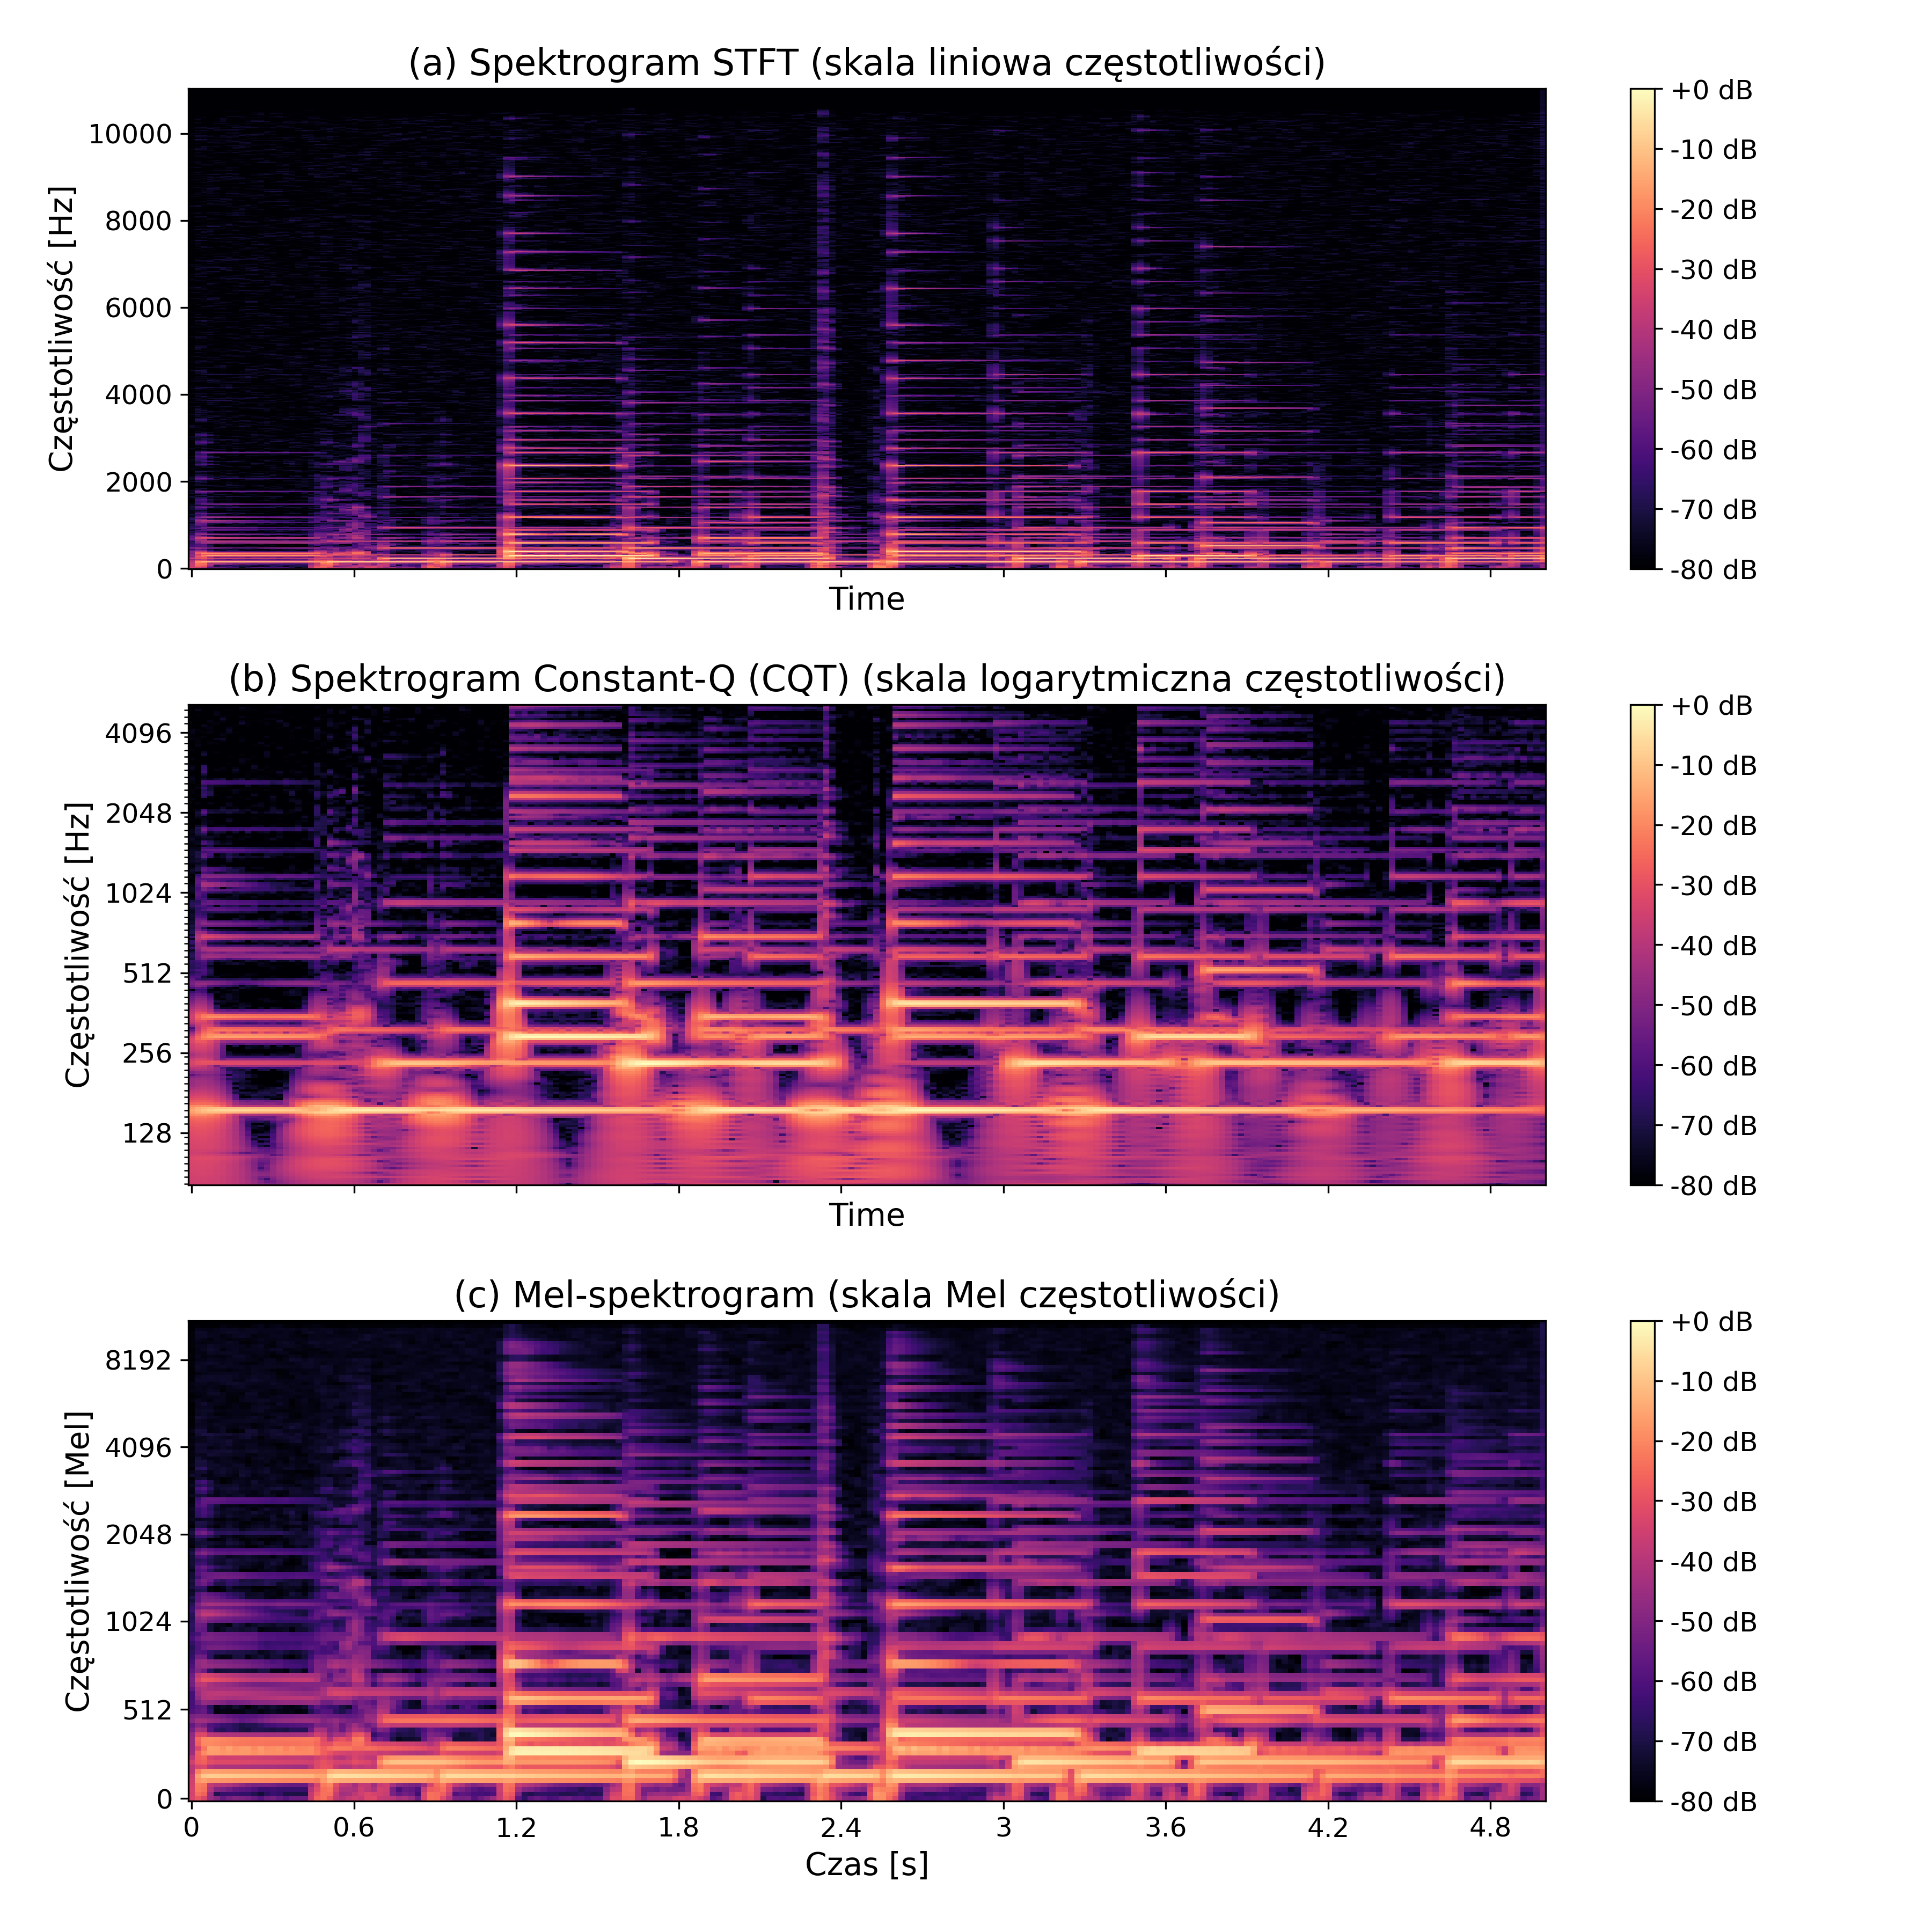
\includegraphics[width=0.85\textwidth]{fig/fig_2_2.png}
    \caption{Wizualizacja różnych reprezentacji czasowo-częstotliwościowych dla tego samego polifonicznego fragmentu gitarowego: (a) Spektrogram STFT z~liniową skalą częstotliwości, (b) Spektrogram Constant-Q (CQT) z~logarytmiczną skalą częstotliwości, (c) Mel-spektrogram z~osią częstotliwości w~skali Mel.}
    \label{fig:fig_2_2}
\end{figure}

\section{Automatyczna transkrypcja muzyczna: zadania, poziomy i wyzwania}
\label{sec:rdzen_atm}

ATM, jest procesem wieloetapowym, obejmującym szereg skomplikowanych zadań cząstkowych. Zrozumienie tych zadań, poziomów abstrakcji, na jakich operują, oraz nieodłącznych wyzwań jest kluczowe dla oceny istniejących rozwiązań i~projektowania nowych.

\subsection{Definicja, zadania składowe i poziomy abstrakcji w ATM}
\label{ssec:definicja_zadania_poziomy_atm}

Formalnie, ATM można zdefiniować jako proces estymacji parametrów nut, takich jak czas rozpoczęcia, wysokość i~czas trwania, bezpośrednio z~sygnału audio~\autocite{KlapuriDavy2006SignalProcessing,Benetos2019AutomaticMusicTranscription}. Jest to zadanie hierarchiczne, które można zdekomponować na kilka kluczowych zadań składowych. Do najważniejszych z~nich należą~\autocite{Benetos2019AutomaticMusicTranscription,Hawthorne2018Onsets}:
\begin{itemize}
    \item \textbf{estymacja wielokrotnej wysokości dźwięku} (ang. \textit{Multiple Pitch Estimation}, MPE), czyli identyfikacja wszystkich częstotliwości podstawowych obecnych w~danym momencie;
    \item \textbf{detekcja początku i~końca dźwięku} (ang. \textit{Onset/Offset Detection}), czyli precyzyjne lokalizowanie w~czasie momentów rozpoczęcia i~zakończenia poszczególnych zdarzeń muzycznych;
    \item \textbf{zadania zaawansowane}, takie jak rozpoznawanie instrumentów, analiza rytmu i~metrum czy interpretacja ekspresji wykonawczej.
\end{itemize}

Wyniki transkrypcji mogą być prezentowane na różnych poziomach abstrakcji~\autocite{Benetos2019AutomaticMusicTranscription}:
\begin{itemize}
    \item \textbf{na poziomie krótkich ramek czasowych}, np. poprzez wskazanie aktywnych wysokości dźwięku w~oknie kilkudziesięciu milisekund;
    \item \textbf{na poziomie symbolicznym}, jako zestaw nut z~określonymi atrybutami;
    \item \textbf{na poziomie strukturalnym}, jako bardziej złożone obiekty, takie jak strumienie melodyczne czy pełna partytura muzyczna.
\end{itemize}

\begin{figure}[!htbp]
    \centering
    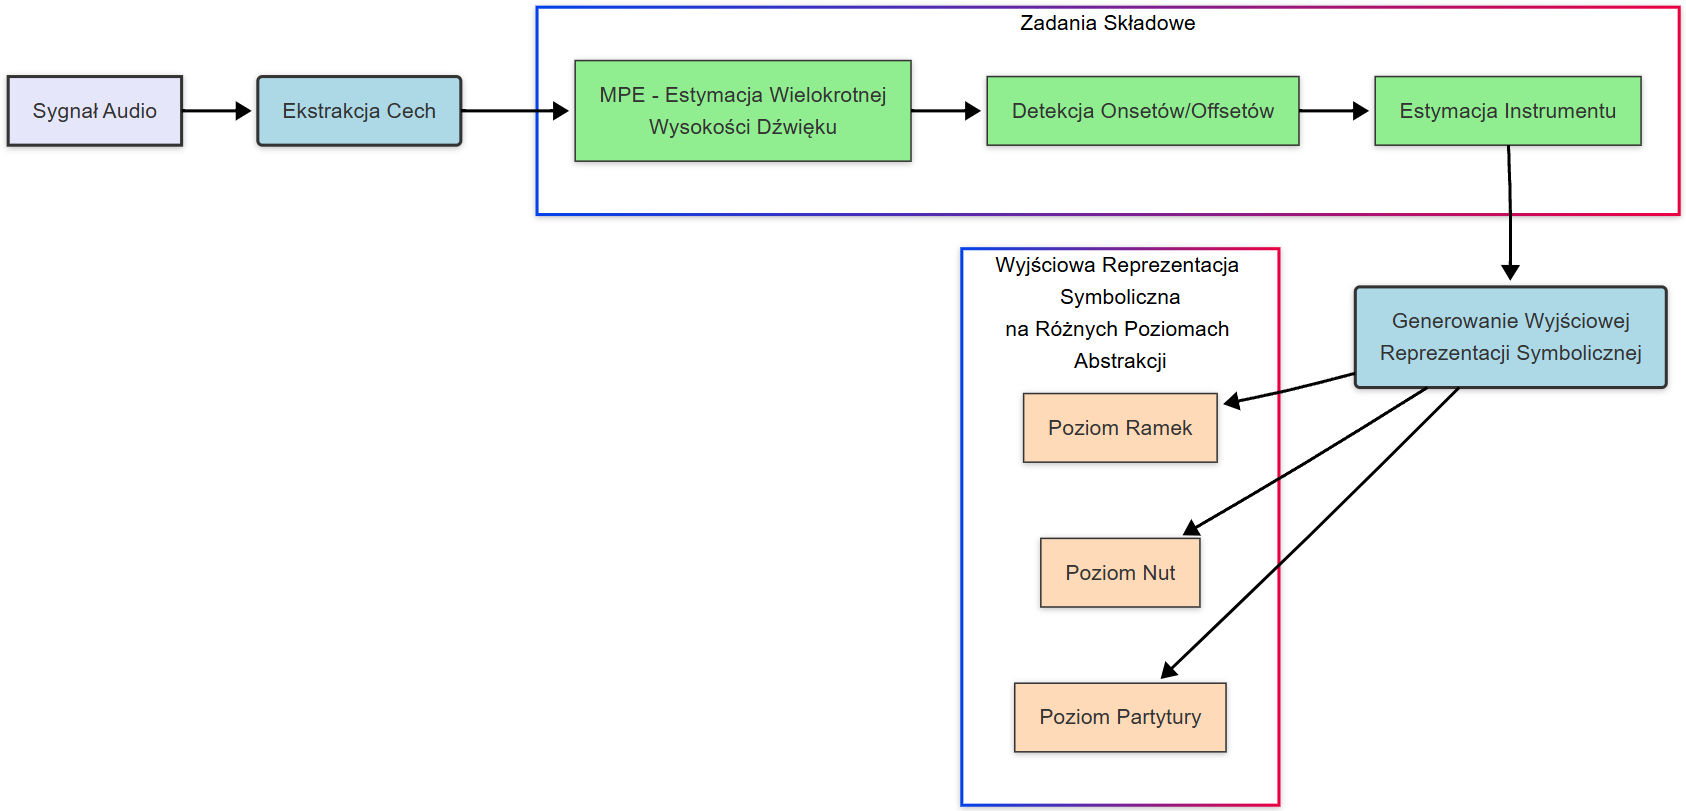
\includegraphics[width=1.0\textwidth]{fig/fig_2_3.png}
    \caption{Uproszczony schemat potoku przetwarzania w~systemie ATM: od sygnału audio, poprzez ekstrakcję cech, zadania składowe (MPE, detekcja onsetów/offsetów, estymacja instrumentu), aż po generowanie wyjściowej reprezentacji symbolicznej na różnych poziomach abstrakcji (ramki, nuty, partytura)~\autocite{Benetos2019AutomaticMusicTranscription}.}
    \label{fig:fig_2_3}
\end{figure}

\subsection{Transkrypcja monofoniczna vs polifoniczna – złożoność i główne wyzwania}
\label{ssec:mono_vs_poli_wyzwania}

Złożoność zadania ATM znacząco wzrasta przy przejściu od transkrypcji monofonicznej (pojedyncza linia melodyczna) do polifonicznej (wiele współbrzmiących dźwięków)~\autocite{KlapuriDavy2006SignalProcessing,Benetos2019AutomaticMusicTranscription}. Muzyka gitarowa, ze względu na możliwość gry akordowej i~prowadzenia wielu niezależnych linii melodycznych, jest w~przeważającej mierze polifoniczna, co czyni jej transkrypcję szczególnie trudną~\autocite{BurletHindle2017IsolatedGuitarTranscription}. Główne wyzwania w~ATM, które ulegają intensyfikacji w~kontekście polifonii, to przede wszystkim: interferencja harmonicznych składowych różnych dźwięków (szczególnie w~interwałach konsonansowych), maskowanie cichszych dźwięków przez głośniejsze, trudności w~precyzyjnej detekcji czasów rozpoczęcia i~zakończenia dźwięków w~gęstych fakturach, zmienność barwy dźwięku zależna od artykulacji i~dynamiki, oraz częste błędy w~estymacji wysokości, takie jak pomyłki oktawowe~\autocite{Benetos2019AutomaticMusicTranscription}. Dodatkowo, efektywne trenowanie modeli uczenia maszynowego wymaga dostępu do dużych, dokładnie zaanotowanych zbiorów danych, których tworzenie jest procesem czasochłonnym i~kosztownym.
%Początek
\section{Przegląd metod stosowanych w automatycznej transkrypcji muzycznej}
\label{sec:przeglad_metod_atm}

Rozwój metod ATM jest procesem ciągłym, odzwierciedlającym postęp w~dziedzinach przetwarzania sygnałów i~uczenia maszynowego. Poniżej przedstawiono ewolucję tych podejść, od metod klasycznych po najnowsze techniki oparte na głębokim uczeniu.

\subsection{Metody tradycyjne oparte na przetwarzaniu sygnałów}
\label{ssec:tradycyjne_metody_cps}

Historycznie pierwsze podejścia do ATM opierały się w~dużej mierze na technikach CPS~\autocite{KlapuriDavy2006SignalProcessing}. W~przypadku transkrypcji muzyki monofonicznej, gdzie w~danym momencie występuje tylko jeden dźwięk, opracowano szereg metod detekcji jego częstotliwości podstawowej ($F_0$). Do klasycznych algorytmów należą te bazujące na analizie funkcji autokorelacji (ang. \textit{Auto-Correlation Function}, ACF), uśrednionej funkcji różnicowej amplitudy (ang. \textit{Average Magnitude Difference Function}, AMDF), technice spektrum harmonicznego iloczynu (ang. \textit{Harmonic Product Spectrum}, HPS), która wzmacnia częstotliwość podstawową poprzez mnożenie widma z~jego wersjami skompresowanymi w~dziedzinie częstotliwości (tj. widmami poddanymi decymacji), oraz na analizie cepstralnej (ang. \textit{cepstral analysis}). Cepstrum, będące wynikiem odwrotnej transformaty Fouriera z~logarytmu widma mocy sygnału, pozwala na separację składowej związanej ze źródłem dźwięku (pobudzeniem) od składowej związanej z~charakterystyką filtru rezonansowego instrumentu~\autocite{KlapuriDavy2006SignalProcessing}. Rozwijano również systemy bazujące na modelach harmonicznych dźwięku oraz systemy ekspertowe, wykorzystujące predefiniowane reguły i~wiedzę muzykologiczną~\autocite{KlapuriDavy2006SignalProcessing}. Metody te wykazywały znaczne ograniczenia w~kontekście analizy muzyki polifonicznej, gdzie jednoczesne występowanie wielu dźwięków i~ich alikwotów znacząco komplikuje sygnał, prowadząc m.in. do niemożności separacji nakładających się szeregów harmonicznych. Ograniczenia te stały się motywacją do poszukiwania bardziej zaawansowanych rozwiązań w~ramach uczenia maszynowego.

\subsection{Metody oparte na uczeniu maszynowym}
\label{ssec:metody_uczenia_maszynowego_atm}

Przełom w~skuteczności systemów ATM przyniosło zastosowanie metod uczenia maszynowego, które pozwoliły na tworzenie modeli zdolnych do nauki złożonych zależności bezpośrednio z~danych~\autocite{Jamshidi2024SurveyAMT,BurletHindle2017IsolatedGuitarTranscription}. W~ramach tego paradygmatu można wyróżnić kilka głównych kierunków.

\subsubsection{Nienadzorowane metody faktoryzacji macierzy}
\label{sssec:nmf_atm}

Wśród metod nienadzorowanych, popularność zdobyła nieujemna faktoryzacja macierzy (ang. \textit{Non-negative Matrix Factorization}, NMF)~\autocite{Benetos2019AutomaticMusicTranscription}. W kontekście muzycznym, technika ta polega na dekompozycji (rozłożeniu) macierzy wejściowej, którą jest spektrogram, na iloczyn dwóch macierzy o mniejszych wymiarach, również posiadających wyłącznie wartości nieujemne.

Pierwsza z nich, \textbf{macierz szablonów} (słownika), zawiera zbiór charakterystycznych profili spektralnych. Każdy taki profil można interpretować jako ``dźwiękowy odcisk palca'' pojedynczej nuty, ukazujący rozkład energii na jej częstotliwość podstawową i kolejne harmoniczne. Druga macierz, \textbf{macierz aktywacji}, określa z kolei, z jaką głośnością i w którym momencie każdy z tych szablonów pojawia się w oryginalnym nagraniu. W ten sposób spektrogram całego utworu jest reprezentowany jako suma ważona podstawowych komponentów muzycznych.

Zaletą NMF jest jej zdolność do automatycznego, nienadzorowanego odkrywania tych fundamentalnych struktur w danych. Istotnym wyzwaniem jest jednak fakt, że podstawowa wersja NMF może mieć trudności z separacją źródeł o silnie nakładających się charakterystykach spektralnych -- na przykład dźwięków w konsonansowych interwałach, których harmoniczne pokrywają się. W celu rozwiązania tych problemów opracowano liczne rozszerzenia NMF, takie jak nadzorowane NMF (gdzie szablony są predefiniowane i stałe) czy harmoniczne NMF (które narzucają harmoniczną strukturę na szablony, zapewniając ich muzyczną poprawność)~\autocite{Benetos2019AutomaticMusicTranscription}.

\subsubsection{Modele probabilistyczne i bayesowskie}
\label{sssec:modele_probabilistyczne_atm}

Ukryte modele Markowa (ang. \textit{Hidden Markov Models}, HMM) były przez wiele lat intensywnie badane i~stosowane w~ATM, głównie ze względu na ich naturalną zdolność do modelowania sekwencyjnego charakteru muzyki~\autocite{KlapuriDavy2006SignalProcessing,Cazau2017HMM,Raphael2002PianoTranscription}. W~typowym podejściu, ukryte stany HMM mogą odpowiadać poszczególnym nutom lub stanom ciszy, a~obserwacje emitowane przez te stany to wektory cech akustycznych wyekstrahowanych z~kolejnych ramek sygnału audio. Prace Raphaela~\autocite{Raphael2002PianoTranscription} stanowią wczesny przykład zastosowania HMM do transkrypcji muzyki fortepianowej, gdzie modelowano proces generowania nut z~uwzględnieniem prawdopodobieństw przejść między nimi. Cazau i~Nuel~\autocite{Cazau2017HMM} eksplorowali różne warianty HMM, w~tym ich integrację z~metodami dekompozycji spektralnej, jak probabilistyczna analiza składowych ukrytych (ang. \textit{Probabilistic Latent Component Analysis}, PLCA), w~celu poprawy jakości transkrypcji, np. poprzez modelowanie trwania nut lub wykorzystanie wiedzy o~tonalności do modelowania przejść harmonicznych. Podejścia bayesowskie, stanowiące szerszą klasę modeli, pozwalają na formalne włączenie do modelu wcześniejszej wiedzy (np. reguł harmonii, typowych progresji akordów) w~postaci rozkładów a~priori. Mimo pewnych sukcesów, modele te często wymagają starannej inżynierii cech i~mogą mieć trudności z~modelowaniem bardzo złożonych zależności w~muzyce polifonicznej.

\subsubsection{Głębokie sieci neuronowe}
\label{sssec:deep_learning_atm}

W ostatnich latach metody oparte na głębokim uczeniu (DL) zdominowały badania nad ATM, osiągając wyniki stanowiące aktualny stan wiedzy w~wielu aspektach tego zadania~\autocite{Benetos2019AutomaticMusicTranscription,Jamshidi2024SurveyAMT}. Zdolność głębokich sieci neuronowych do automatycznego uczenia się hierarchicznych, wielopoziomowych reprezentacji cech bezpośrednio z~danych wejściowych (np. surowych spektrogramów) okazała się kluczowa dla postępu. Wśród najczęściej wykorzystywanych architektur znajdują się konwolucyjne sieci neuronowe (ang. \textit{Convolutional Neural Networks}, CNN), efektywnie przetwarzające dane o~strukturze siatki, takie jak spektrogramy~\autocite{Wiggins2019TabCNN,Zang2023SynthTab}; rekurencyjne sieci neuronowe (ang. \textit{Recurrent Neural Networks}, RNN), w~szczególności warianty z~długą krótkotrwałą pamięcią (ang. \textit{Long Short-Term Memory}, LSTM) i~bramkowanymi jednostkami rekurencyjnymi (ang. \textit{Gated Recurrent Unit}, GRU), przystosowane do modelowania zależności czasowych w~sekwencjach muzycznych~\autocite{Benetos2019AutomaticMusicTranscription}; oraz architektury hybrydowe, takie jak konwolucyjno-rekurencyjne sieci neuronowe (ang. \textit{Convolutional Recurrent Neural Network}, CRNN), łączące zalety obu tych podejść~\autocite{Hawthorne2018Onsets}. Najnowsze badania eksplorują również potencjał architektur opartych na mechanizmach uwagi, takich jak Transformer (ang. \textit{Transformer})~\autocite{Jamshidi2024SurveyAMT,Hawthorne2021Seq2SeqTranscription}.
Dostępność dużych, publicznych zbiorów danych adnotowanych, takich jak MAESTRO dla muzyki fortepianowej~\autocite{Hawthorne2018Onsets,Zang2023SynthTab} (zawierający nagrania z~konkursów pianistycznych wraz z~odpowiadającymi im plikami MIDI) oraz GuitarSet dla muzyki gitarowej~\autocite{Wiggins2019TabCNN,Zang2023SynthTab,Benetos2019AutomaticMusicTranscription} (oferujący nagrania z~sześciu osobnych przetworników dla każdej struny oraz zsynchronizowane adnotacje MIDI i~tabulaturowe), była katalizatorem rozwoju modeli DL. To właśnie te obszerne i~zaanotowane zbiory danych umożliwiły trenowanie złożonych modeli DL na skalę niezbędną do osiągnięcia wysokiej dokładności, podkreślając, że postęp w~tej dziedzinie jest równie mocno zależny od inżynierii danych, co od innowacji algorytmicznych. Model ,,Onsets and Frames''~\autocite{Hawthorne2018Onsets}, zaprojektowany do transkrypcji muzyki fortepianowej, jest przykładem systemu DL, który osiągnął wysoką skuteczność. Wykorzystuje on architekturę CRNN do jednoczesnej predykcji czasów rozpoczęcia dźwięków (ang. \textit{onsets}) oraz aktywności poszczególnych nut w~kolejnych ramkach czasowych. ,,Basic Pitch''~\autocite{Bittner2022BasicPitch} to z~kolei narzędzie typu audio-to-MIDI, opracowane przez Spotify, które charakteryzuje się lekkością i~zdolnością do detekcji zmian wysokości dźwięku (ang. \textit{pitch bends}). Opiera się na modelach CNN, a~jego priorytetem jest szybkość działania i~dostępność, co czyni je użytecznym w~wielu praktycznych zastosowaniach, chociaż może nie osiągać takiej samej szczegółowości transkrypcji jak bardziej złożone systemy w~przypadku skomplikowanych fragmentów polifonicznych. Mimo imponujących wyników, metody DL nie są pozbawione ograniczeń. Ich skuteczność jest silnie uzależniona od ilości i~jakości danych treningowych, a~trening i~inferencja złożonych modeli DL mogą być wymagające obliczeniowo~\autocite{Jamshidi2024SurveyAMT}.

%Koniec
\section{Specyfika transkrypcji muzyki gitarowej na zapis tabulaturowy (GTT)}
\label{sec:specyfika_gtt}

Transkrypcja muzyki gitarowej, zwłaszcza z~celem wygenerowania zapisu tabulaturowego, wprowadza szereg specyficznych problemów i~wymagań, które odróżniają ją od ogólnego zadania ATM. Niniejsza sekcja poświęcona jest analizie tych unikalnych aspektów.

\subsection{Akustyczna charakterystyka sygnału gitary i jej implikacje dla transkrypcji}
\label{ssec:akustyka_gitary_gtt}

Sygnał generowany przez gitarę posiada szereg unikalnych cech akustycznych, które czynią jego automatyczną transkrypcję zadaniem szczególnie złożonym~\autocite{Wiggins2019TabCNN,BurletHindle2017IsolatedGuitarTranscription}. Obwiednia dźwięku gitary, zwłaszcza akustycznej, charakteryzuje się zazwyczaj bardzo szybkim atakiem i~relatywnie długim, stopniowym wybrzmiewaniem, co może utrudniać precyzyjną detekcję czasów zakończenia dźwięków (ang. \textit{offsets}). Barwa dźwięku gitary jest niezwykle zróżnicowana i~zależy od wielu czynników, takich jak konstrukcja instrumentu (np. gitara akustyczna z~pudłem rezonansowym, gitara elektryczna typu \textit{solid-body}), rodzaj i~wiek strun, technika artykulacji (np. gra kostką, palcami, techniką \textit{slap}), a~w~przypadku gitar elektrycznych~– w~decydującym stopniu od ustawień wzmacniacza oraz zastosowanych efektów gitarowych (np. \textit{distortion, overdrive, chorus, flanger, delay, reverb})~\autocite{Wiggins2019TabCNN}. Ta nieodłączna zmienność i~bogactwo barwowe, choć stanowią o~atrakcyjności instrumentu, komplikują proces tworzenia uogólnionych modeli transkrypcyjnych. Kluczowe dla GTT jest również adekwatne uwzględnienie licznych, specyficznych dla gitary technik wykonawczych, których manifestacje akustyczne przedstawia Tabela~\ref{tab:techniki_gitarowe_latex_poprawiona}. Techniki te nie tylko znacząco wpływają na charakterystykę sygnału, ale także mają swoje bezpośrednie odzwierciedlenie w~zapisie tabulaturowym.

\begin{longtable}{|p{0.18\textwidth}|p{0.39\textwidth}|p{0.33\textwidth}|}
    \caption[Wybrane techniki gitarowe i ich manifestacje akustyczne]{Akustyczne manifestacje wybranych technik gitarowych istotnych dla transkrypcji na tabulaturę.}
    \label{tab:techniki_gitarowe_latex_poprawiona} \\
    \hline
    \textbf{Technika} & \textbf{Opis} & \textbf{Akustyczna Manifestacja (Przykładowa)} \\
    \hline
    \endfirsthead
    \hline
    \textbf{Technika} & \textbf{Opis} & \textbf{Akustyczna Manifestacja (Przykładowa)} \\
    \hline
    \endhead
    \hline
    \endfoot
    \hline
    \endlastfoot
    (ang. \textit{Hammer-on}) & Uderzenie palcem lewej ręki (dla praworęcznych gitarzystów) w~strunę na wyższym progu w~celu wydobycia dźwięku bez ponownego szarpania struny prawą ręką.
    & Zazwyczaj łagodniejszy atak spektralny w~porównaniu do dźwięku szarpniętego; możliwy spadek amplitudy po wykonaniu techniki, szczególnie na cieńszych strunach~\autocite{Nasution2023HammerOn};
    poprzedzający dźwięk (jeśli był) może wybrzmiewać w~tle z~niższą amplitudą~\autocite{Nasution2023HammerOn,Su2014SparseCepstral}.
    Brak wyraźnego ,,dołka'' w~amplitudzie między nutami w~sekwencji legato~\autocite{Reboursiere2011GuitarController}.
    \\
    \hline
    (ang. \textit{Pull-off}) & Oderwanie palca lewej ręki od struny (zazwyczaj z~lekkim jej szarpnięciem) w~celu wydobycia niższego dźwięku, który już brzmi (np. na pustej strunie lub przytrzymywany innym palcem na niższym progu).
    & Podobnie jak \textit{hammer-on}, charakteryzuje się łagodniejszym atakiem w~porównaniu do dźwięku szarpniętego; zmiana wysokości następuje na niższą;
    może towarzyszyć krótki, szerokopasmowy szum związany z~mechanicznym ruchem odrywania palca~\autocite{Su2014SparseCepstral}.
    \\
    \hline
    (ang. \textit{Slide}) (ślizg) & Płynne przesunięcie palca lewej ręki wzdłuż struny pomiędzy dwoma progami, podczas gdy struna wibruje.
    & Ciągła, płynna zmiana częstotliwości podstawowej ($F_0$) i~jej harmonicznych (tzw. \textit{glissando}) między wysokością początkową a~końcową~\autocite{Su2014SparseCepstral,Reboursiere2011GuitarController};
    zachowanie energii sygnału i~jego ciągłości spektralnej; charakterystyczny profil przejścia między wysokościami, odróżniający od techniki \textit{bend}~\autocite{Su2014SparseCepstral}.
    \\
    \hline
    (ang. \textit{Bend}) (podciągnięcie) & Poprzeczne podciągnięcie struny na gryfie palcem lewej ręki, co zwiększa jej napięcie i~w~rezultacie podwyższa wysokość dźwięku.
    & Płynna zmiana wysokości dźwięku ($F_0$) w~górę, często z~następującym powrotem do oryginalnej wysokości lub przejściem do innej~\autocite{Su2014SparseCepstral,Reboursiere2011GuitarController};
    mogą pojawić się charakterystyczne zmiany w~natężeniu alikwotów oraz subtelne zmiany barwy.
    \\
    \hline
    (ang. \textit{Palm-muting}) & Delikatne tłumienie strun krawędzią dłoni prawej ręki (dla gitarzystów praworęcznych) w~pobliżu mostka gitary, bezpośrednio po ich szarpnięciu.
    & Znaczne skrócenie czasu wybrzmiewania dźwięku (szybszy zanik energii); stłumiony, bardziej perkusyjny i~mniej rezonujący charakter;
    redukcja udziału wyższych harmonicznych w~spektrum, co prowadzi do ,,ciemniejszego'', ,,cichszego'' brzmienia~\autocite{Su2014SparseCepstral}.
    \\
    \hline
    (ang. \textit{Vibrato}) & Cykliczna, subtelna modulacja wysokości dźwięku, uzyskiwana przez oscylacyjny ruch palca przytrzymującego strunę na progu lub za pomocą ramienia tremolo.
    & Okresowe, stosunkowo wolne (typowo 5-7 Hz) fluktuacje częstotliwości podstawowej ($F_0$) i~jej harmonicznych wokół centralnej wysokości dźwięku~\autocite{Anand2012Vibrato,HyrkasSmyth2024Vibrato};
    może również występować sprzężona z~tym modulacja amplitudy~\autocite{Anand2012Vibrato,HyrkasSmyth2024Vibrato}.
    \\
\end{longtable}

\subsection{Porównanie notacji standardowej i tabulaturowej dla gitary}
\label{ssec:porownanie_notacji_gitara}

W praktyce muzycznej gitarzyści posługują się dwoma głównymi systemami notacji: tradycyjną notacją muzyczną opartą na pięciolinii oraz tabulaturą gitarową. Każdy z~tych systemów posiada swoje unikalne cechy, które determinują jego adekwatność w~różnych zastosowaniach i~dla różnych grup użytkowników~\autocite{Wiggins2019TabCNN}. Tabela~\ref{tab:porownanie_notacji_latex} przedstawia zwięzłe porównanie obu systemów. Wybór tabulatury jako docelowej formy zapisu w~wielu współczesnych systemach GTT jest motywowany jej dużą popularnością, zwłaszcza wśród gitarzystów samouków i~w~muzyce rozrywkowej, oraz jej bezpośrednim, instruktażowym charakterem, który ułatwia naukę i~wykonanie utworu na instrumencie.

\begin{table}[H]
    \centering
    \caption{Porównanie standardowej notacji muzycznej i~tabulatury gitarowej.}
    \label{tab:porownanie_notacji_latex}
    \begin{tabular}{|p{0.2\textwidth}|p{0.38\textwidth}|p{0.32\textwidth}|}
        \hline
        \textbf{Cecha} & \textbf{Standardowa Notacja Muzyczna} & \textbf{Tabulatura Gitarowa} \\
        \hline
        Reprezentacja wysokości & Abstrakcyjna, poprzez pozycję nuty na pięciolinii, wymagająca znajomości klucza i~zasad teorii muzyki~\autocite{Wiggins2019TabCNN}.
        & Bezpośrednia, poprzez wskazanie numeru progu na linii reprezentującej konkretną strunę gitary~\autocite{Wiggins2019TabCNN}.
        \\
        \hline
        Reprezentacja rytmu & Precyzyjnie zdefiniowana za pomocą wartości rytmicznych nut, pauz i~oznaczeń metrycznych~\autocite{Wiggins2019TabCNN}.
        & Często uproszczona lub nieobecna; główny nacisk kładziony jest na wysokość i~sposób opalcowania. Rytm bywa jednak dodawany za pomocą symboli podobnych do notacji standardowej lub poprzez odniesienie do nagrania~\autocite{Wiggins2019TabCNN}.
        \\
        \hline
        Czytelność dla gitarzystów & Wymaga dłuższego procesu nauki i~praktyki w~czytaniu nut na pięciolinii~\autocite{Wiggins2019TabCNN}.
        & Zazwyczaj bardzo intuicyjna i~łatwa do szybkiego opanowania, szczególnie dla początkujących gitarzystów i~samouków; bezpośrednio pokazuje, gdzie umieścić palce na gryfie~\autocite{Wiggins2019TabCNN}. \\
        \hline
        Notacja technik gry & Możliwa za pomocą licznych dodatkowych symboli i~oznaczeń słownych, ale czasami może być mniej jednoznaczna lub intuicyjna dla specyficznych technik gitarowych.
        & Bardzo dobrze przystosowana do notowania szerokiego spektrum specyficznych technik gitarowych (np. \textit{bends, slides, hammer-ons, pull-offs, vibrato}) za pomocą dedykowanych symboli graficznych.
        \\
        \hline
        Niejednoznaczność opalcowania & Istnieje~– ten sam dźwięk (wysokość) może być zagrany na gitarze na kilku różnych strunach i~progach; wybór konkretnego opalcowania jest pozostawiony wykonawcy~\autocite{Wiggins2019TabCNN}. & Zazwyczaj jednoznacznie określa zarówno strunę, jak i~próg, na którym dany dźwięk ma być zagrany, tym samym eliminując problem wyboru opalcowania dla danej nuty~\autocite{Wiggins2019TabCNN}.
        \\
        \hline
    \end{tabular}
\end{table}

\subsection{Kluczowe wyzwania w automatycznej transkrypcji gitary na tabulaturę (GTT)}
\label{ssec:wyzwania_gtt}

Transkrypcja na tabulaturę wprowadza szereg specyficznych wyzwań, które wykraczają poza ogólne problemy ATM:
\begin{itemize}
    \item \textbf{Wysoka polifonia i~nakładanie się dźwięków}: Gitara, jako instrument harmoniczny, często generuje złożone współbrzmienia, co intensyfikuje problem separacji i~identyfikacji poszczególnych dźwięków w~sygnale audio~\autocite{BurletHindle2017IsolatedGuitarTranscription}.
    \item \textbf{Niejednoznaczność reprezentacji dźwięku na gryfie} (ang. \textit{Tablature Inference / Fingering Estimation}): Jest to jedno z~fundamentalnych wyzwań w~GTT. Ten sam dźwięk (o tej samej wysokości muzycznej) może być zagrany w~wielu różnych pozycjach na gryfie gitary (tj. na różnych kombinacjach struny i~progu)~\autocite{Wiggins2019TabCNN}. Wybór konkretnej pozycji przez gitarzystę zależy od wielu czynników, takich jak kontekst muzyczny (np. sąsiednie dźwięki), grywalność (łatwość wykonania danego pochodu dźwięków), preferencje stylistyczne, a~nawet subtelne różnice w~barwie dźwięku uzyskiwane na różnych strunach. System GTT musi więc nie tylko poprawnie zidentyfikować wysokość i~czas trwania nuty, ale również podjąć decyzję co do jej najbardziej prawdopodobnego i/lub optymalnego opalcowania na gryfie. Ilustruje to rysunek~\ref{fig:fig_2_4}.
    \begin{figure}[H]
        \centering
        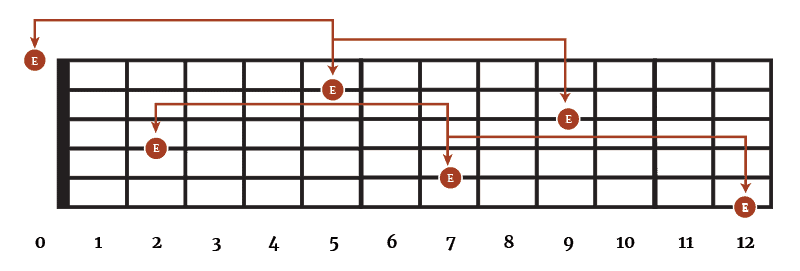
\includegraphics[width=0.6\textwidth]{fig/fig_2_4.png}
        \caption{Przykład tej samej nuty (E4, MIDI 64) możliwej do zagrania w~wielu pozycjach na gryfie gitary standardowo strojonej. Ilustracja przedstawia dźwięk E4 na strunie G (9.~próg), strunie B (5.~próg) oraz pustej strunie wysokiej E. Obrazuje to wyzwanie estymacji opalcowania w~GTT~\autocite{obrazGitaraNiejednoznacznosc}.}
        \label{fig:fig_2_4}
    \end{figure}
    \item \textbf{Zmienność barwy jako potencjalna wskazówka i~problem}: Chociaż subtelne różnice w~barwie dźwięku tej samej nuty granej na różnych strunach mogą teoretycznie dostarczać pewnych wskazówek dla algorytmów estymacji opalcowania, to wszechobecne i~często intensywne stosowanie efektów gitarowych (szczególnie w~muzyce rockowej, metalowej, jazzowej i~elektronicznej) może całkowicie modyfikować oryginalną barwę instrumentu, maskując te subtelne różnice lub wprowadzając własne artefakty, co znacząco komplikuje analizę~\autocite{Wiggins2019TabCNN}.
    \item \textbf{Detekcja i~notacja technik wykonawczych}: Wierne odtworzenie partii gitarowej w~formie tabulatury wymaga nie tylko transkrypcji samych nut, ale również rozpoznania i~odpowiedniego zanotowania licznych, specyficznych dla gitary technik artykulacyjnych (patrz Tabela~\ref{tab:techniki_gitarowe_latex_poprawiona})~\autocite{Reboursiere2011GuitarController,Su2014SparseCepstral}. Jest to zadanie trudne, gdyż akustyczne manifestacje tych technik bywają subtelne i~zmienne.
    \item \textbf{Problem ,,przesunięcia dziedziny''} (ang. \textit{domain shift}): Modele GTT trenowane na danych pochodzących z~jednej domeny (np. czyste, studyjne nagrania gitar akustycznych lub dane syntetyczne) mogą wykazywać znaczący spadek skuteczności, gdy są stosowane do danych z~innej domeny (np. nagrania koncertowe, amatorskie, partie gitar elektrycznych z~efektami)~\autocite{Zang2023SynthTab}. Praca Zang i~współpracowników~\autocite{Zang2023SynthTab} nad zbiorem SynthTab stanowi próbę zaadresowania problemu niedoboru zróżnicowanych danych rzeczywistych poprzez wykorzystanie dużych ilości danych syntetycznych do wstępnego treningu modeli, które następnie mogą być dostrajane na mniejszych zbiorach danych rzeczywistych.
\end{itemize}


\subsection{Przegląd istniejących podejść i narzędzi do GTT}
\label{ssec:podejscia_narzedzia_gtt}

Współczesne podejścia do GTT można generalnie podzielić na dwuetapowe oraz zintegrowane, określane jako (ang. \textit{end-to-end}). Podejścia dwuetapowe realizują zadanie GTT w~dwóch oddzielnych krokach: najpierw dokonuje się ogólnej transkrypcji MPE, a~następnie w~osobnym kroku (inferencji opalcowania) przypisuje się wykryte nuty do pozycji na gryfie~\autocite{BurletHindle2017IsolatedGuitarTranscription}. Zaletą tego podejścia jest jego modularność, a~wadą ryzyko propagacji błędów z~pierwszego etapu.

Podejścia zintegrowane, opierające się w~przeważającej mierze na zaawansowanych modelach DL, dążą do nauczenia się bezpośredniego mapowania z~reprezentacji czasowo-częstotliwościowej na finalną reprezentację tabulaturową. Wykorzystują one złożone architektury sieci neuronowych, takie jak:
\begin{itemize}
    \item Modele oparte na CNN, czego przykładem jest TabCNN~\autocite{Wiggins2019TabCNN}. Architektura ta typowo przetwarza wejściowy spektrogram (np. Constant-Q) i~generuje na wyjściu predykcje dotyczące aktywności poszczególnych progów na każdej ze strun gitary, często w~formacie wielowymiarowej macierzy binarnej (tzw. ,,six-hot encoding''). Praca Zang i~współpracowników~\autocite{Zang2023SynthTab} również wykorzystuje architekturę zbliżoną do TabCNN jako jeden z~modeli bazowych w~swoich badaniach nad wykorzystaniem danych syntetycznych.
    \item Modele oparte na architekturze Transformer, które dzięki zastosowaniu mechanizmów uwagi (ang. \textit{attention mechanisms}) są zdolne do efektywnego modelowania długoterminowych zależności w~danych sekwencyjnych. Znalazły one zastosowanie w~GTT, szczególnie w~połączeniu z~dużymi zbiorami danych, w~tym syntetycznymi, takimi jak SynthTab~\autocite{Zang2023SynthTab}.
    \item Inne architektury, w~tym RNN (np. LSTM czy GRU), często stosowane w~połączeniu z~CNN (tworząc architektury CRNN), aby wykorzystać zdolności CNN do ekstrakcji lokalnych cech ze spektrogramów oraz zdolności RNN do modelowania kontekstu czasowego~\autocite{BurletHindle2017IsolatedGuitarTranscription}. Przykładowo, praca Burlet i~Hindle~\autocite{BurletHindle2017IsolatedGuitarTranscription} badała zastosowanie głębokich sieci przekonań (ang. \textit{Deep Belief Networks}) dla transkrypcji izolowanych dźwięków gitarowych, co stanowiło wczesny przykład wykorzystania metod DL w~tym obszarze.
\end{itemize}
Zaletą podejść zintegrowanych jest ich potencjalna zdolność do uczenia się bardzo złożonych i~subtelnych mapowań bezpośrednio z~danych, co może prowadzić do lepszych wyników końcowych niż w~podejściach dwuetapowych. Wymagają one jednak zazwyczaj znacznie większych i~bardziej szczegółowych zbiorów danych treningowych. Niezależnie od podejścia, kluczową rolę w~rozwoju systemów GTT odgrywają zbiory danych, które zostaną szerzej omówione w~kolejnych rozdziałach.

\section{Podsumowanie i otwarte problemy badawcze}
\label{sec:podsumowanie_analizy_gtt}

Automatyczna transkrypcja muzyczna, a~w~jej ramach transkrypcja muzyki gitarowej na zapis tabulaturowy, pozostaje aktywnym i~wymagającym obszarem badań naukowych. Znaczenie praktyczne skutecznych systemów GTT jest nie do przecenienia, obejmując wsparcie dla muzyków, edukację, archiwizację oraz przemysł muzyczny~\autocite{Benetos2019AutomaticMusicTranscription}. Analiza przeprowadzona w~niniejszym rozdziale wykazała, że główne wyzwania koncentrują się wokół przetwarzania złożonych sygnałów polifonicznych, radzenia sobie z~dużą zmiennością barwy i~artykulacji charakterystyczną dla gitary, a~w~przypadku GTT~– dodatkowo wokół problemu niejednoznaczności opalcowania oraz detekcji i~notacji specyficznych technik wykonawczych~\autocite{Wiggins2019TabCNN}.

Przegląd stosowanych metod ukazuje wyraźną ewolucję od klasycznych technik opartych na przetwarzaniu sygnałów do zaawansowanych modeli uczenia maszynowego, które obecnie definiują stan wiedzy w~tej dziedzinie~\autocite{KlapuriDavy2006SignalProcessing,Jamshidi2024SurveyAMT}. Rozwiązania takie jak ,,Onsets and Frames''~\autocite{Hawthorne2018Onsets} czy ,,Basic Pitch''~\autocite{Bittner2022BasicPitch} dla ogólnych zadań ATM, oraz systemy dedykowane GTT, jak TabCNN~\autocite{Wiggins2019TabCNN} i~nowsze podejścia wykorzystujące duże zbiory danych, w~tym syntetyczne, jak w~przypadku badań nad SynthTab~\autocite{Zang2023SynthTab}, demonstrują znaczący postęp. Mimo to, wciąż istnieją liczne obszary wymagające dalszych, intensywnych badań. Do kluczowych otwartych problemów w~dziedzinie GTT, które wyznaczają kierunki przyszłych prac, należą przede wszystkim:
\begin{enumerate}
    \item Dalsza poprawa dokładności i~odporności transkrypcji w~kontekście gęstych faktur polifonicznych, szybkich pasaży muzycznych oraz sygnałów o~niskiej jakości lub z~silnymi zniekształceniami.
    \item Rozwój bardziej zaawansowanych i~kontekstowych metod inferencji opalcowania na gryfie gitary, które lepiej odzwierciedlałyby rzeczywiste praktyki wykonawcze i~zapewniały grywalność generowanych tabulatur.
    \item Zwiększenie zdolności systemów do rozpoznawania i~poprawnej notacji szerokiego spektrum technik gitarowych, które mają kluczowe znaczenie dla ekspresji muzycznej.
    \item Poprawa generalizacji modeli GTT na różne, nie widziane wcześniej w~procesie treningu, brzmienia gitar (akustycznych, elektrycznych, z~różnymi efektami), style muzyczne i~warunki nagraniowe.
    \item Opracowanie bardziej kompleksowych i~percepcyjnie adekwatnych metryk oceny jakości transkrypcji tabulaturowej, które wykraczałyby poza proste porównanie poprawności nut i~uwzględniałyby aspekty takie jak grywalność, czytelność i~wierność stylistyczną. Kwestia ta nawiązuje do obserwacji, że wyniki ilościowe nie zawsze w~pełni odzwierciedlają praktyczną użyteczność systemu dla końcowego użytkownika~\autocite{Holzapfel2019Ethnomusicology}.
    \item Kontynuacja prac nad tworzeniem i~udostępnianiem większych, bardziej zróżnicowanych i~precyzyjnie adnotowanych zbiorów danych dla GTT, w~tym eksploracja metod efektywnego wykorzystania danych syntetycznych i~technik transferu wiedzy.
\end{enumerate}

Niniejsza praca magisterska stanowi próbę odpowiedzi na niektóre z~wymienionych wyzwań. W~kolejnych rozdziałach przedstawiony zostanie projekt i~implementacja systemu, który w~szczególności skupia się na problemach wyszczególnionych w~punktach (1) i~(2), czyli na poprawie ogólnej dokładności transkrypcji oraz rozwoju metod inferencji opalcowania.